\documentclass[../master]{subfiles}

\begin{document}

\chapter{MAIKo TPC}
\section{MAIKo TPC とは}
我々のグループでは低エネルギー荷電粒子を大立体角で検出するために,
アクティブ標的TPC であるMAIKo TPC~\cite{MAIKo}を開発してきた.
MAIKo TPC は検出ガスを封入する密封容器 (MAIKo チェンバー) と
ドリフト電場を形成するケージ(ドリフトケージ)からなる.
図\ref{fig::maiko_cage}および図\ref{pic::MAIKo_cage}にドリフトケージの模式図と写真を示す.
ドリフトケージはMAIKo チェンバー内に設置して用いる.
図\ref{fig::MAIKo_view}にMAIKo TPC 中で入射中性子と${}^{12}\mathrm{C}$の散乱によって,
${}^{12}\mathrm{C} (0_2^+)$から放出された3つの$\alpha$粒子と取得されるトラック画像との対応を示す.
MAIKo TPC では荷電粒子のトラックを$zy$平面と$xy$平面の2つの2次元平面に射影した画像
(anode imageとcathode image) として得られる.
また,電荷を持たない中性子のトラックは検出されない.
MAIKo TPC は検出ガスを標的ガスとして用いるアクティブ標的であるため,
$\alpha$粒子を大立体角で検出することができる.

TPC は荷電粒子のトラックを検出するために広く用いられているガス検出器である.
図\ref{fig::drift_electrons}にTPC でトラックを検出するイメージを示す.
荷電粒子がTPC の検出ガス中を通過するとき,トラックの周囲の粒子をイオン化させる.
イオン化で発生した電子をドリフト電場 (図\ref{fig::drift_electrons}中で上向き) により読み出し面にドリフトさせる.
読み出し面に電子が到達した時間を記録し,記録された時間差からドリフト方向の距離を測定する.
さらに,2次元平面でドリフトしてきた電子の位置を測定することで,3次元的にトラックを検出できる.
MAIKo TPC では3次元のトラックを2つの平面に射影した画像として取得する.
%読み出し平面を2つの軸で独立して測定するため,2つの2次元画像として得られる.
%
%TPC の有感領域中で入射粒子と標的粒子が散乱することで,
%散乱点の周りを有感領域で覆うことができるため,
%散乱で放出される低エネルギーの荷電粒子を大立体角で検出することが可能となる.
%図\ref{fig::MAIKo_view}は検出器中で入射中性子と${}^{12}\mathrm{C}$との散乱によって,
%3つの$\alpha$粒子が放出されたイベント表す.
%有感領域中で散乱することで,3つの$\alpha$粒子を全て検出できる.
%これを実現する方法として,検出器そのものを標的として用いるアクティブ標的がある.
%アクティブ標的を用いたTPC として我々はMAIKo TPC を開発した.
%MAIKo TPC,は検出ガスを封入する密封容器 (MAIKo チェンバー) と
%ドリフト電場を形成するケージ (ドリフトケージ) とからなる.
%ドリフトケージを図\ref{pic::MAIKo_cage}に,
%%MAIKo チェンバーを図\ref{pic::MAIKo_chamber}に示す.
%%ドリフトケージはMAIKo チェンバー内に設置して用いる.
\begin{figure}
  \centering
  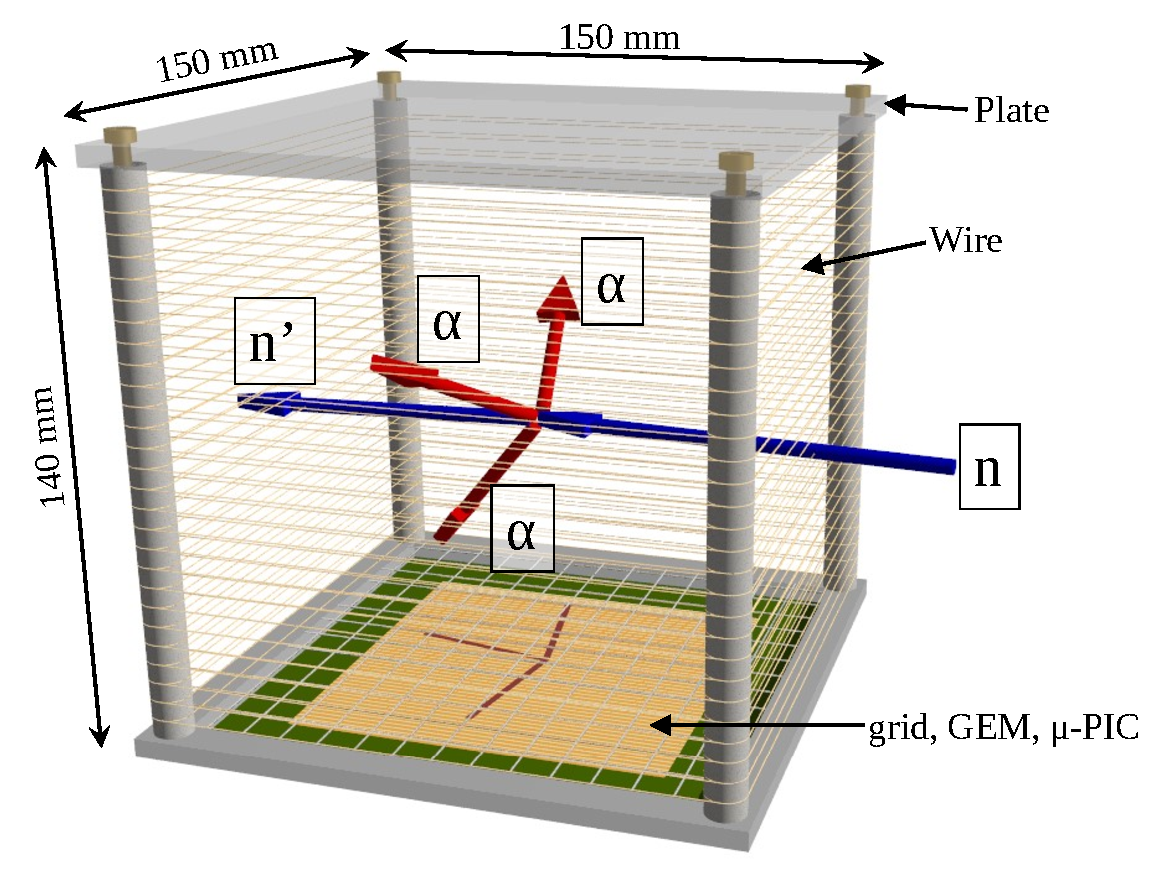
\includegraphics[clip, width=0.65\columnwidth]{maiko.pdf}
  \caption{MAIKo TPC の概観図.
    検出ガスに含まれる${}^{12}\mathrm{C}$が右から入射した中性子(青色)と散乱し
    3つの$\alpha$粒子に崩壊したときを模している.}
  \label{fig::maiko_cage}
\end{figure}
\begin{figure}
  \centering
  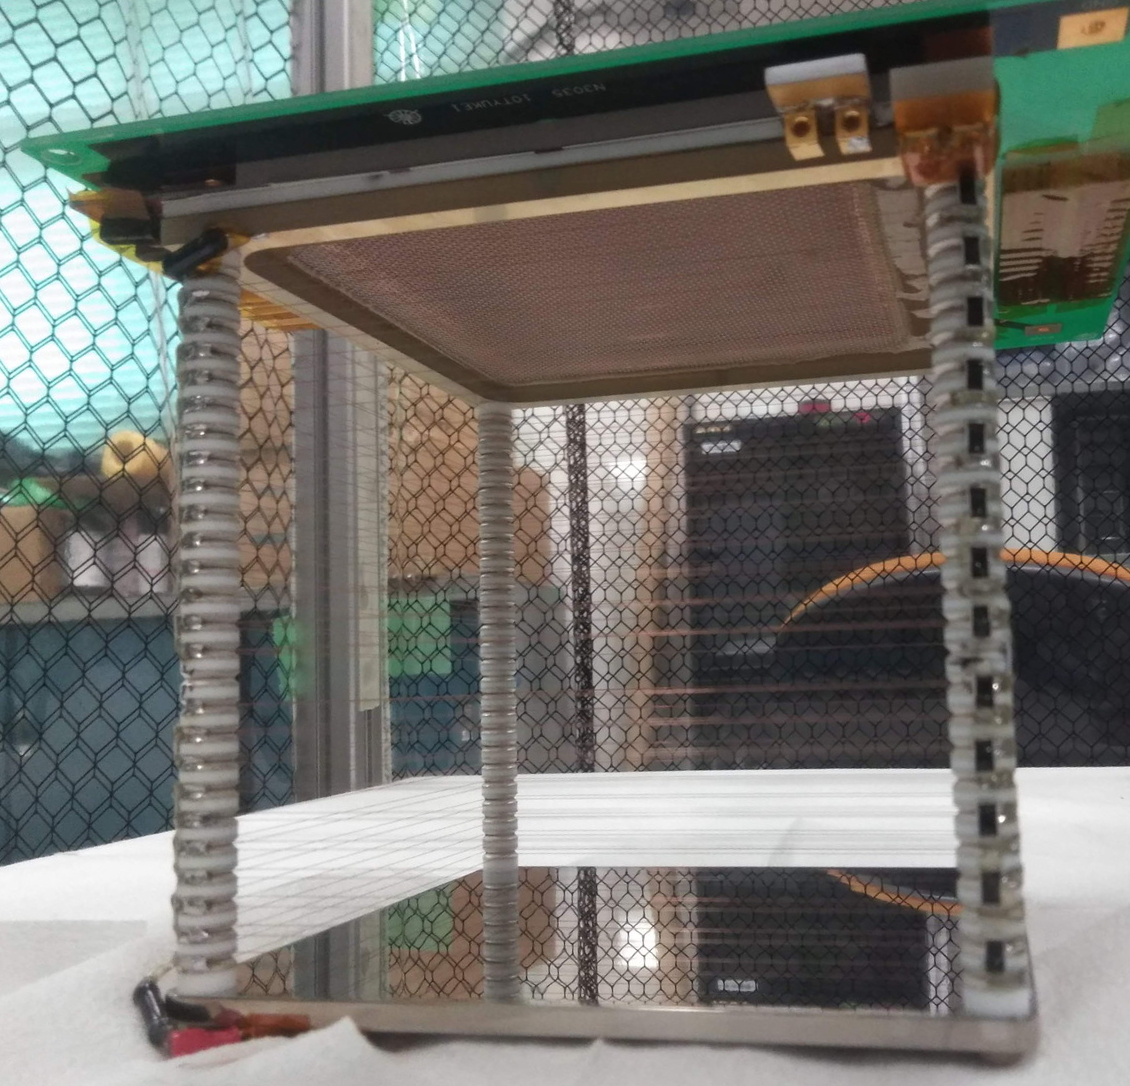
\includegraphics[clip, width=0.6\columnwidth]{IMG_20190731_110230_clpd.jpg}
%  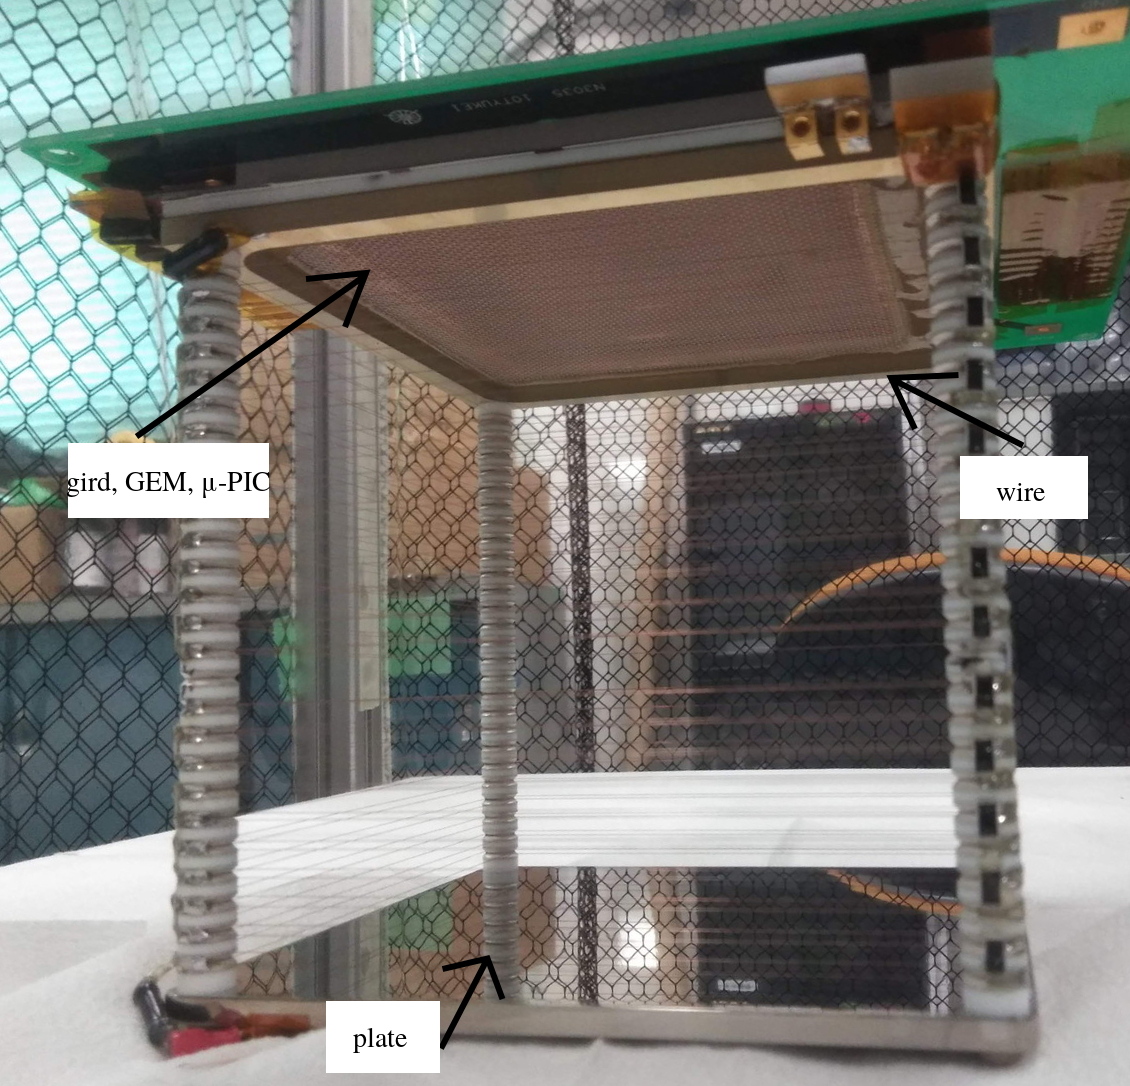
\includegraphics[clip, width=0.8\columnwidth]{IMG_20190731_110230_drwd.jpg}
  \caption[ドリフトケージの概観.]
          {ドリフトケージの概観.ケージの上側に読み出し面が取り付けられている.
          図\ref{fig::maiko_cage}および図\ref{fig::MAIKo_view}とは上下が反転している.}
  \label{pic::MAIKo_cage}
\end{figure}
\begin{figure}
  \centering
  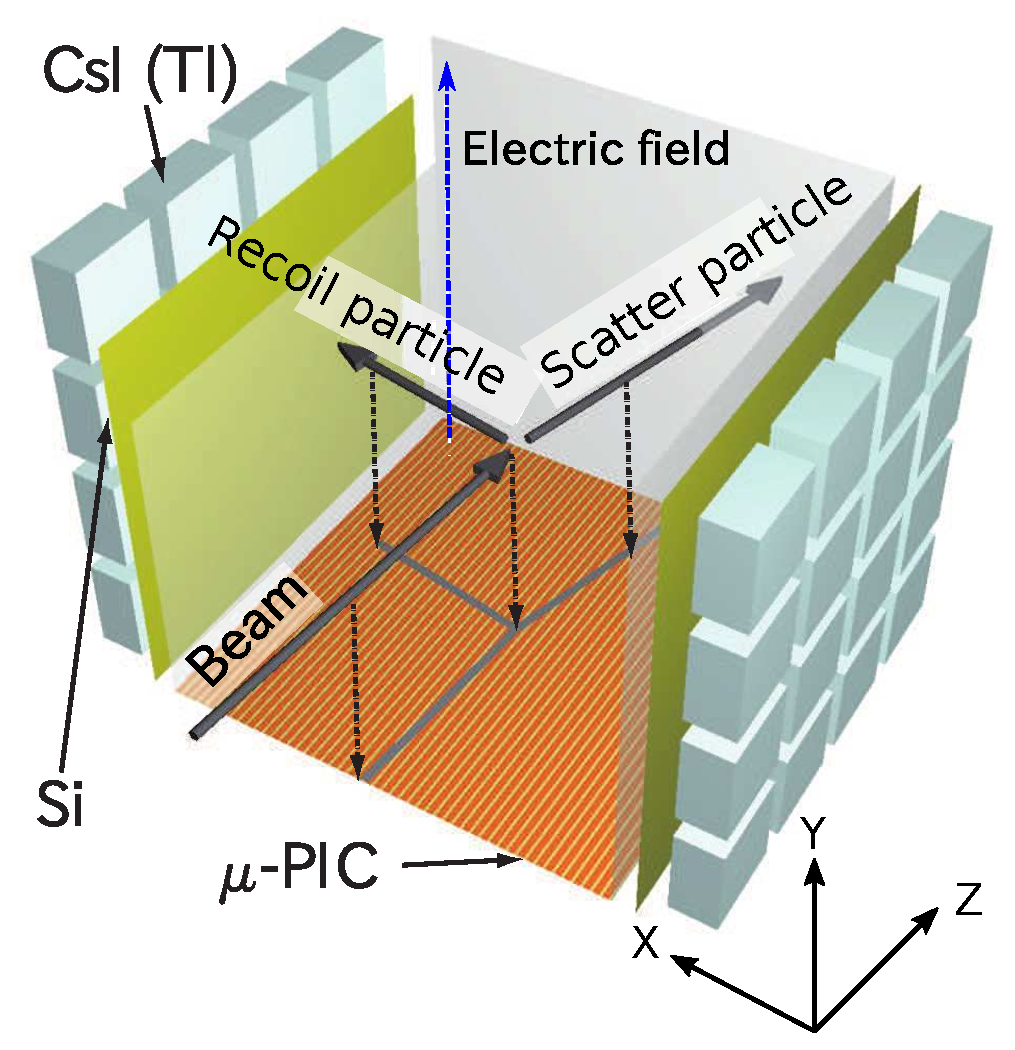
\includegraphics[clip, width=0.8\columnwidth]{MAIKo.eps}
  \caption{MAIKo TPC で取得される画像と実際の荷電粒子のトラックとの対応.
    図ではTPC の中の${}^{12}\mathrm{C}$が右から入射した中性子 (青) と散乱し,
    3つの$\alpha$粒子 (赤) に崩壊した事象を表す.
    anode image ($zy$平面) と cathode image ($xy$平面) の2平面に荷電粒子のトラックが射影される(茶色の線).
    中性子は電荷を持たないためanode,cathode image にトラックとして検出されない.
  }
  \label{fig::MAIKo_view}
\end{figure}
\begin{figure}
  \centering
  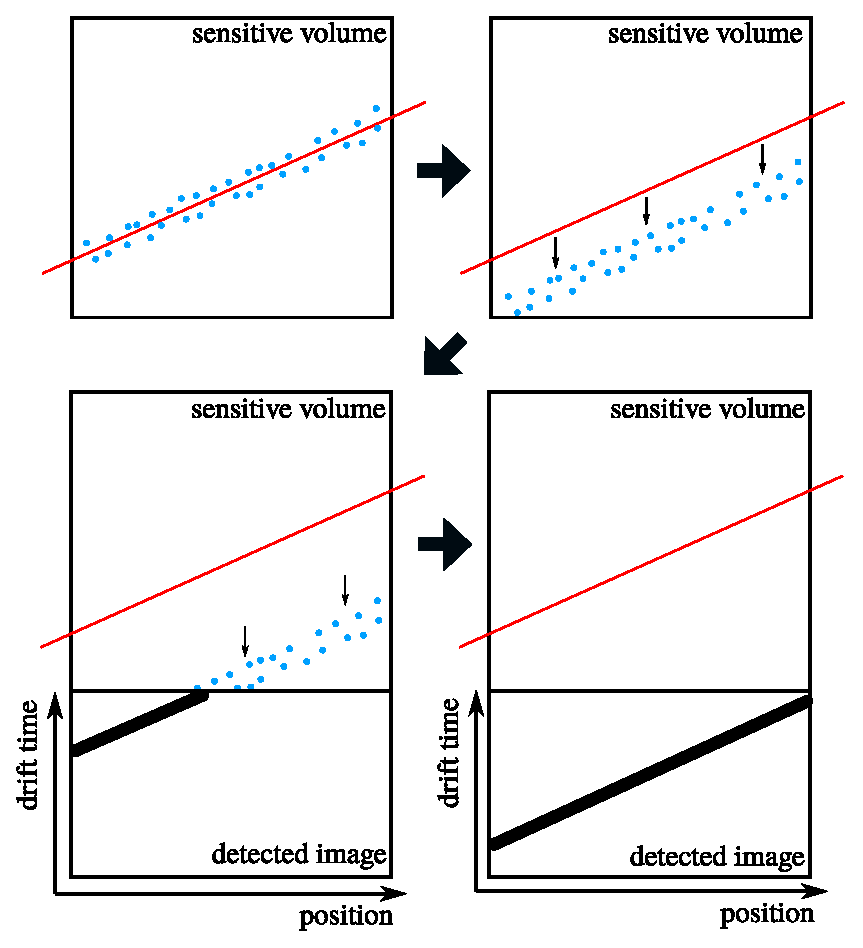
\includegraphics[clip, width=0.9\columnwidth]{drift_electrons.eps}
  \caption{TPC でトラックを検出するときのイメージ.
    赤い実線は荷電粒子のトラック,青い点はイオン化で生成された電子,
    黒く太い実線は検出されたトラックを表す.
    トラックは電子が読み出し面に到達した時間として記録される.}
  \label{fig::drift_electrons}
\end{figure}
%\begin{figure}
%  \centering
%  \begin{subfigure}{0.45\columnwidth}
%    \centering
%    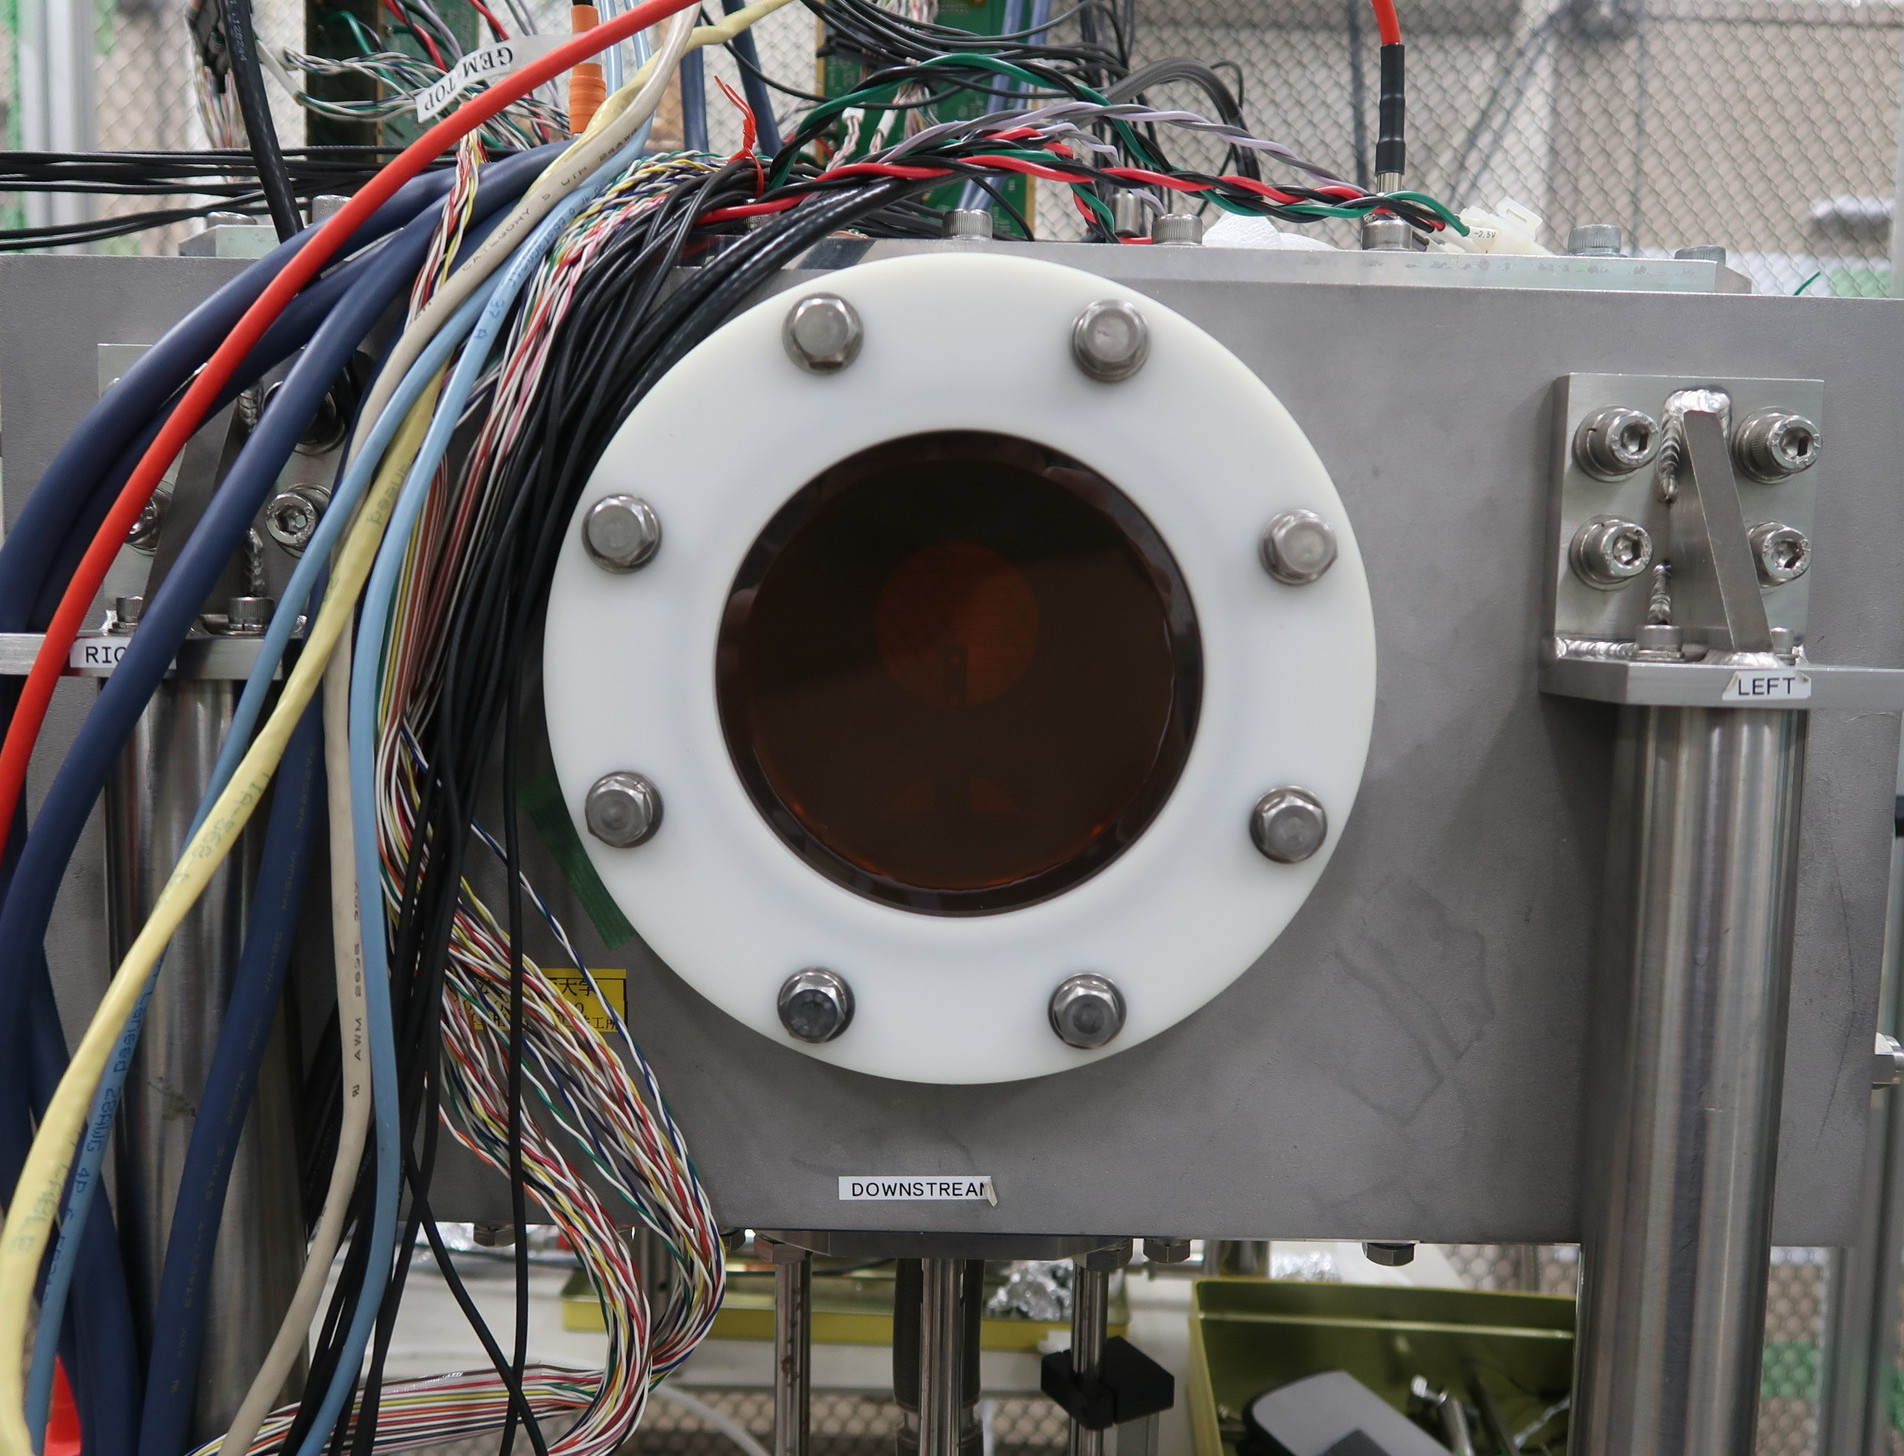
\includegraphics[clip, width=\columnwidth]{IMG_2925_clpd.jpg}
%    \caption{外側.}
%    \label{pic::MAIKo_chamber_out}
%  \end{subfigure}
%  \begin{subfigure}{0.45\columnwidth}
%    \centering
%    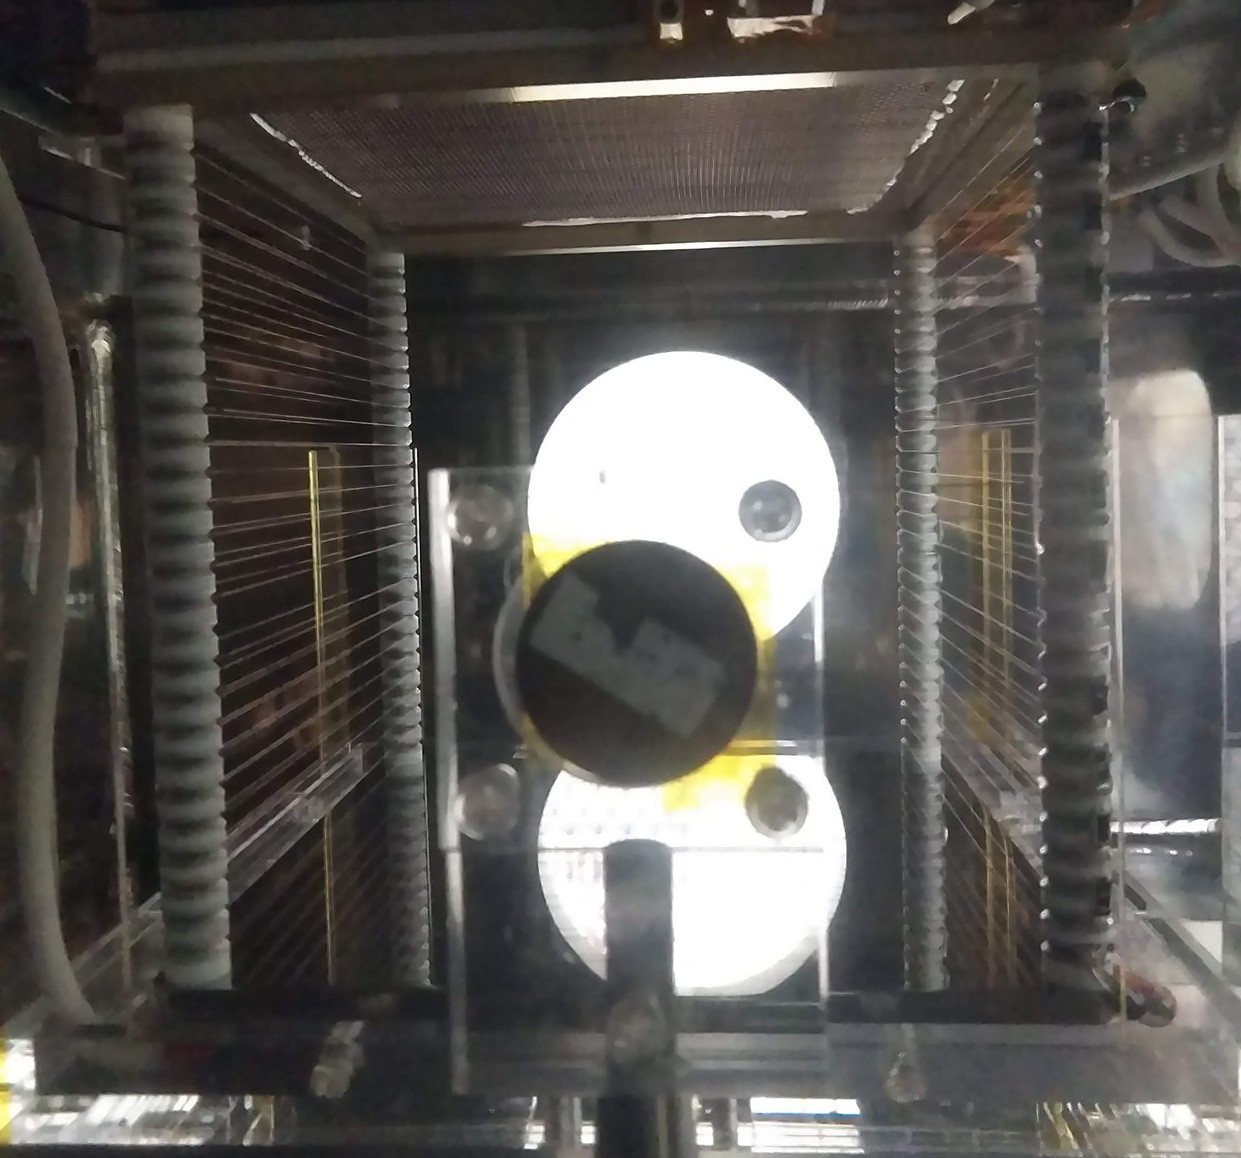
\includegraphics[clip, width=\columnwidth]{IMG_20190801_160046_clpd.jpg}
%    \caption{内側.}
%    \label{pic::MAIKo_chamber_in}
%  \end{subfigure}
%  \caption{MAIKo チェンバー.}
%  \label{pic::MAIKo_chamber}
%\end{figure}

図\ref{fig::MAIKo_cage}にドリフトケージの構造を示す.
ドリフトケージはplate,wire,grid,gas electron multiplier (GEM),$\mu$-PIC~\cite{mupic}からなる.
plate,grid,GEM,$\mu$-PICに高圧電源 (HV) が接続されている.
plate,wire,girdの間は\SI{10}{\mega\ohm}の抵抗で繋がれている.
GEM とHV は\SI{1}{\mega\ohm}と\SI{20}{\mega\ohm}の抵抗で繋がれている.
plateからgridの間の領域(ドリフト領域)で発生した電子がgrid に向かってドリフトし,
gridから$\mu$-PICの間の領域(増幅領域)にあるGEM と$\mu$-PICによって増幅され,
$\mu$-PIC(読み出し領域)によって増幅された電子の2次元位置を読み出す.
ドリフト領域は$y$軸方向に\SI{140}{\milli\metre}であり,
読み出し面の大きさが\SI{102.4x102.4}{\milli\metre}であるので,
有感領域の大きさは\SI{102.4x102.4x140}{\milli\metre}となる.
\begin{figure}
  \centering
  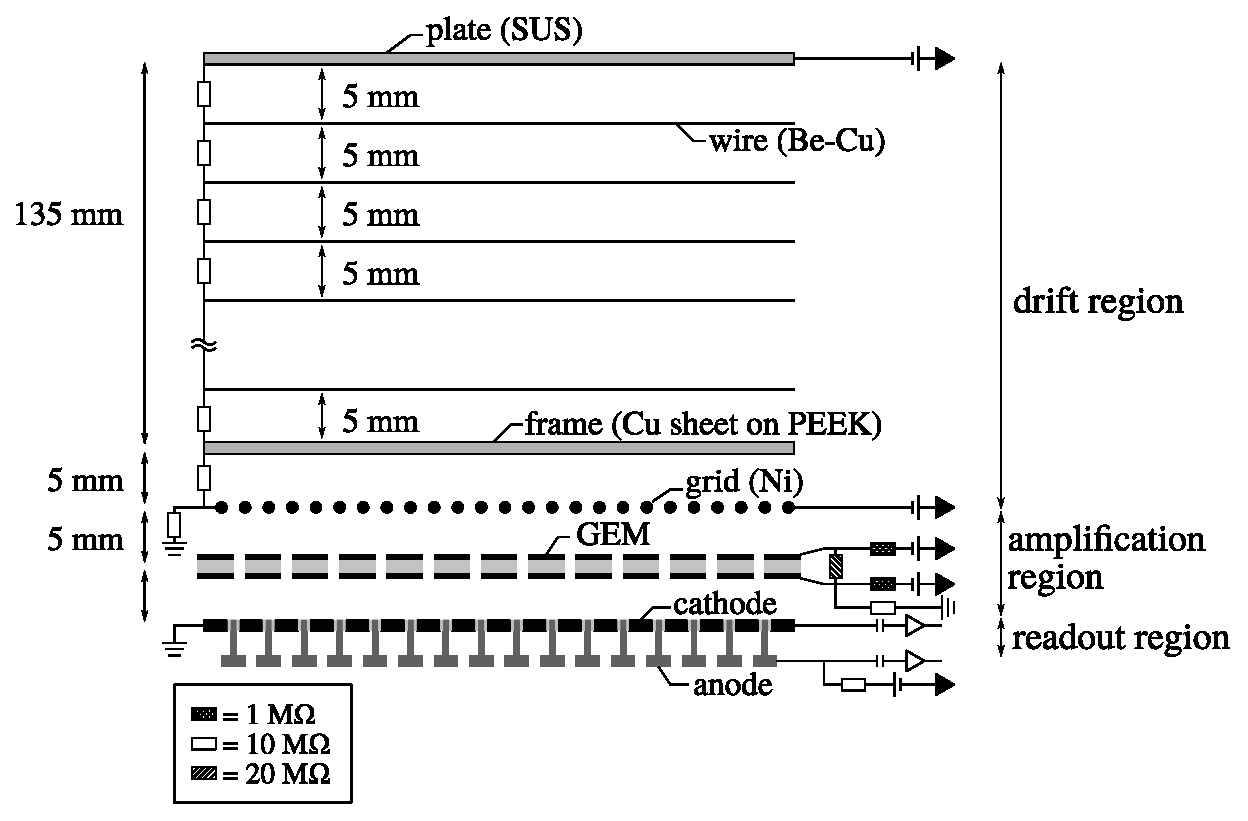
\includegraphics[clip, width=\columnwidth]{MAIKo_cage.eps}
  \caption{ドリフトケージの構造.}
  \label{fig::MAIKo_cage}
\end{figure}

%plate とgrid に電圧をかけることでドリフト領域にドリフト電場を形成する.
%ドリフト領域を荷電粒子が通過する際に生成された電子がドリフト電場によって増幅領域へ移動する.
%ドリフト電場を一様に形成するために5 mm間隔でドリフト領域の周囲にwire を巻いてある.
%ドリフト領域はドリフト方向に140 mm である.
%ドリフトしてきた電子は,まずGEM (gas electron multiplier) で増幅される.
%増幅した電子およびイオンによって$\mu$-PIC のanode とcathode に誘起された信号を読み出す.
%$\mu$-PIC では信号の読み出しだけでなく電子の増幅も行われる.

\subsection{ドリフト領域}
plate とgrid にそれぞれ高電圧を印加することでドリフト電場を形成し,
grid からplate の方向 (図\ref{fig::MAIKo_cage}では上向き) にドリフト電場を形成することで
入射した荷電粒子の周囲に発生した電子を増幅領域へドリフトさせる.
ドリフト電場の一様性が高いほど,トラックの周囲に発生した電子雲の形状を保ったまま,
電子をドリフトさせることができる.
均等にドリフトしない場合,正しくトラックを検出することができなくなってしまう.
ドリフト電場を一様に形成するために\SI{10}{\mega\ohm}の抵抗で接続された直径\SI{125}{\micro\metre}のBe-Cu wire が
\SI{5}{\milli\metre}間隔で二重で巻かれている~\cite{furuno}.

\subsection{増幅領域}
MAIKo TPC ではGEM と$\mu$-PICを用いて電子の増幅を行う.
GEM は,図\ref{pic::GEM}のようにポリマーのフィルムの表面を銅で被覆し,
直径\SI{70}{\micro\metre} の穴を\SI{140}{\micro\metre}間隔で\SI{1}{\square\milli\metre}あたり
100 個の密度で開けたものである.
銅の2つの層はポリマーによって絶縁されている.
銅の両面に電圧を印加することによって,穴の中に高電場が形成されドリフトしてきた電子が穴を通過する際に増幅される.
MAIKo TPC では厚さ\SI{100}{\micro\metre}の約\SI{100x100}{\milli\metre}のGEM を用いている.
\begin{figure}
  \centering
  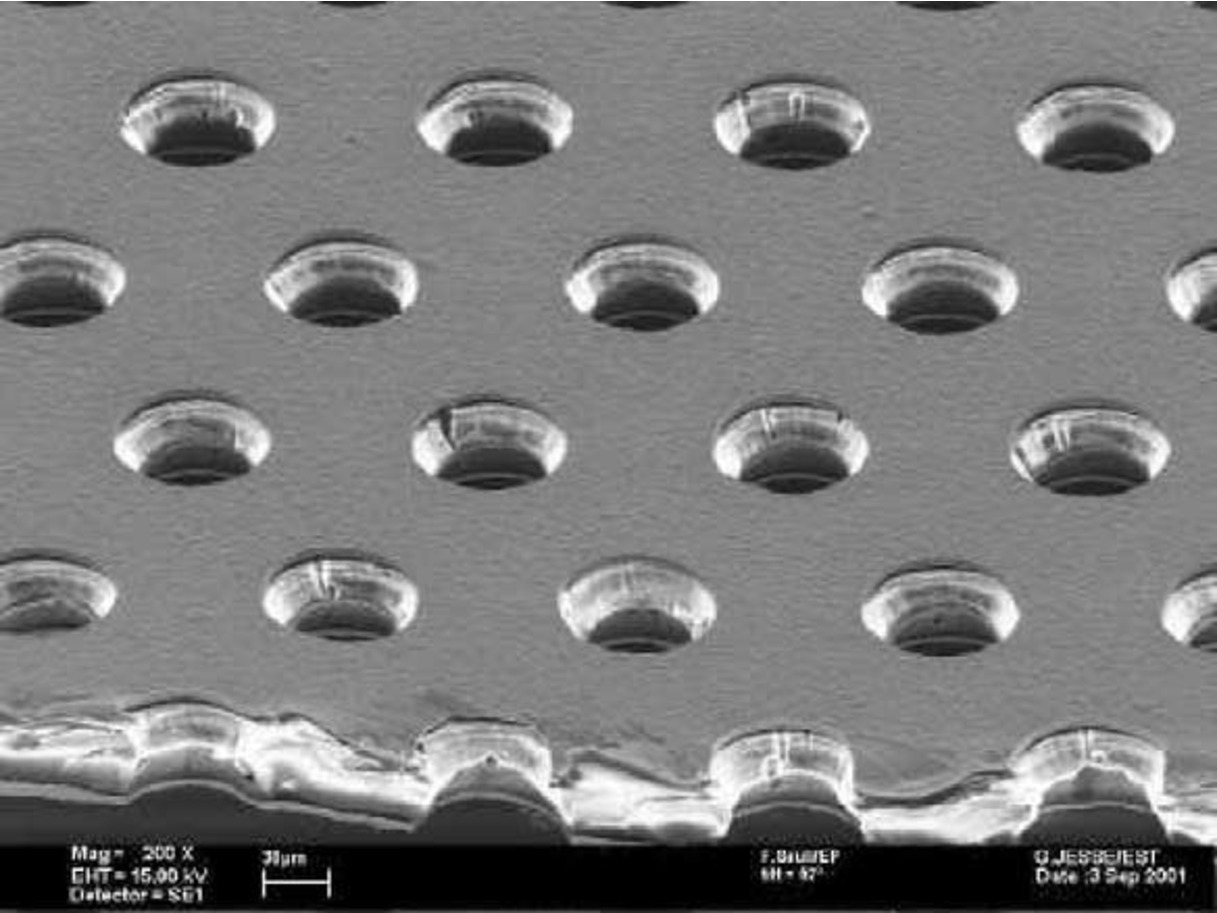
\includegraphics[clip, width=0.7\columnwidth]{gem_structure.pdf}
  \caption{COMPASS 実験で用いられたGEM の拡大図~\cite{gem_compass}.}
  \label{pic::GEM}  
\end{figure}

$\mu$-PIC~\cite{mupic} は京都大学宇宙線研究室で開発されたMicro Pattern Gas Detector の一種である.
$\mu$-PIC は図\ref{fig::mupic}のようにanode strip とcathode strip が直交するように配置されている.
anode strip,cathode strip ともに\SI{400}{\micro\metre}間隔でそれぞれ256~ch分割されている.
直径\SI{50}{\micro\metre}の円柱状のanode 電極に高電圧を印加し,
cathode 電極を接地することでanode 電極付近に強い電場を形成することができ,
GEM で増幅された電子が$\mu$-PICによって更に増幅される.
\begin{figure}
  \centering
  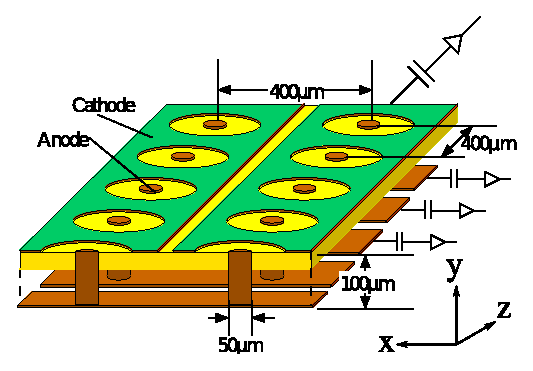
\includegraphics[clip, width=0.7\columnwidth]{upic_struc_xyz.eps}
  \caption[$\mu$-PICの概観図.]{$\mu$-PICの概観図~\cite{mupic}.
    図中の横方向にanode strip,奥行き方向にcathode strip が配置されている.
  }
  \label{fig::mupic}
\end{figure}

\subsection{読み出し領域}
\label{sec::mu-pic}
図\ref{fig::MAIKo_view}と図\ref{fig::mupic}中ではanode strip が$x$軸,cathode strip が$z$軸と平行になるように
$\mu$-PICが配置されている.
GEMと$\mu$-PICにより増幅された電子とイオンをanode strip とcathode strip により読み出すことで,
$z$座標,$x$座標を検出することができる.
また,anode strip とcathode strip で検出される信号の時間分布により$y$座標を決定することができる.

MAIKo TPC からは図\ref{fig::MAIKo_view}のようにトラックが
anode strip に垂直な面 ($zy$平面) に射影されたanode image と
cathode strip に垂直な面 ($xy$平面) に射影されたcathode image の2つの画像が取得される.
MAIKo TPC から得られる画像の1例を図\ref{fig::track_demo}に示す.
anode strip とcathode strip はそれぞれ256~chで構成され,
各ストリップの信号は\SI{100}{\mega\hertz}で1,024~samples測定し,
信号波形が設定した閾値よりも高い場合に1,
低い場合に0として記録される.
%に対するtime over threshold (TOT) を取得する.
%TOT は閾値以上を1,以下を0としたものである.
よって,出力されるデータは解像度が$256\times1,014$~pixels の白黒画像となる.
また,anode strip,cathode strip ともに32~chごとにまとめた信号の波形を
\SI{25}{\mega\hertz}のサンプリング率を持つFADC で取得している.
FADC で取得した信号の一例を図\ref{fig::FADC_waveform}に示す.
\begin{figure}
  \centering
%  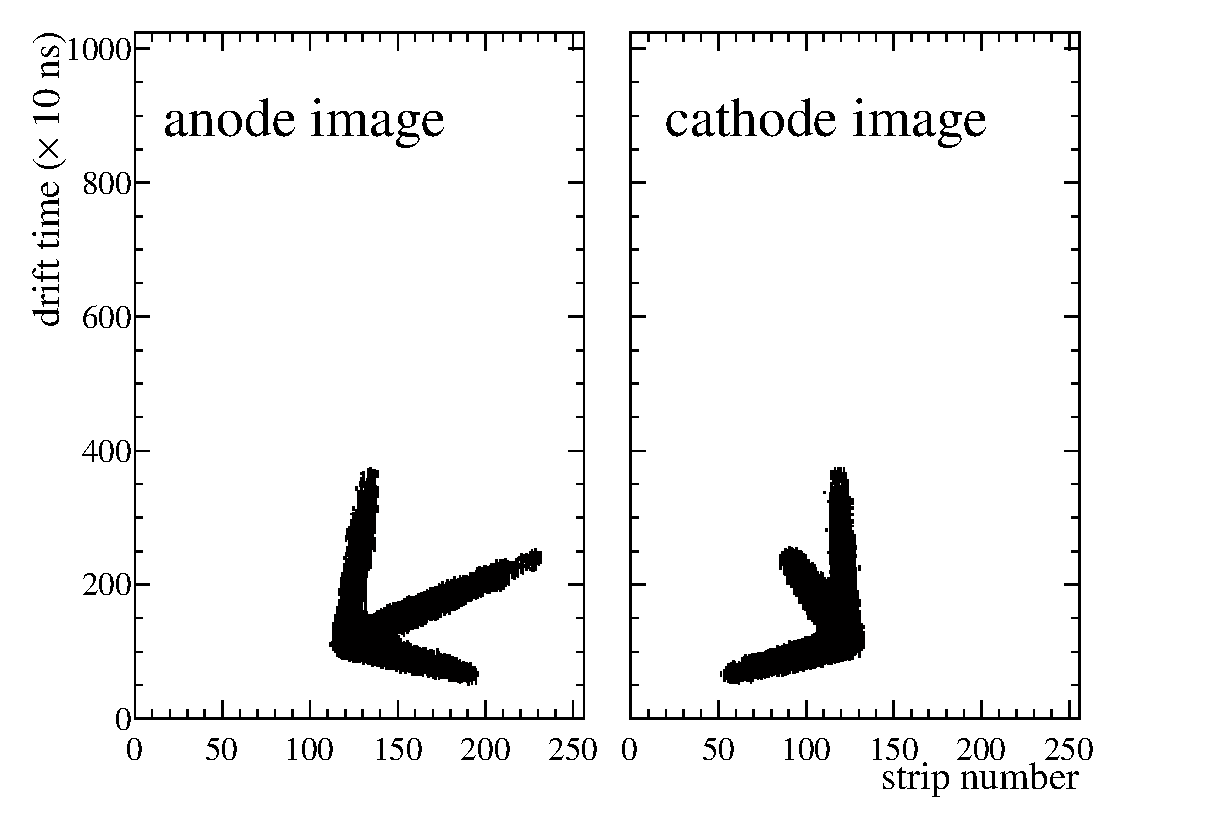
\includegraphics[clip, width=0.9\columnwidth]{10024_4.eps}
  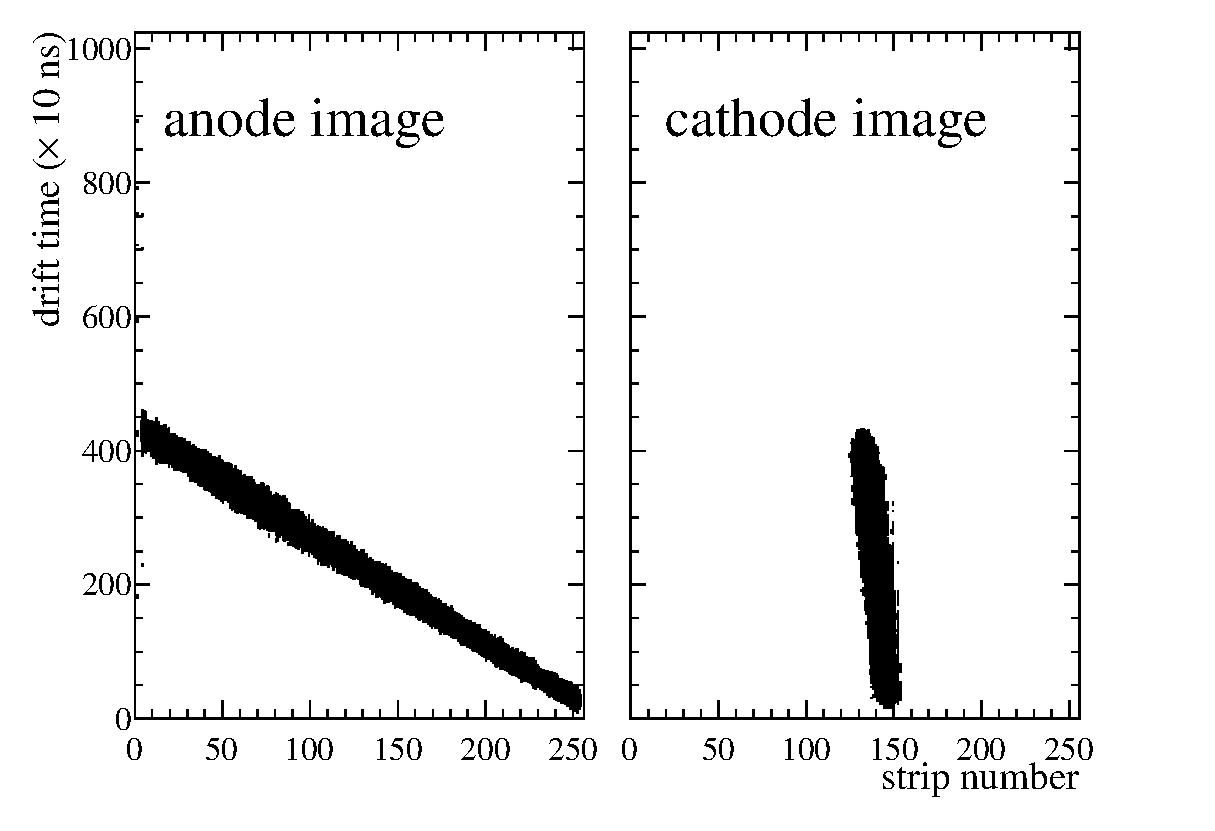
\includegraphics[clip, width=0.8\columnwidth]{0176_1.eps}
  \caption[MAIKo TPC から得られる画像データの一例.]
          {MAIKo TPC から得られる画像データの一例.
          このイベントは\ref{chap::simulation}章で述べる線源を用いて測定したデータである.}
  \label{fig::track_demo}
\end{figure}
\begin{figure}
  \centering
%  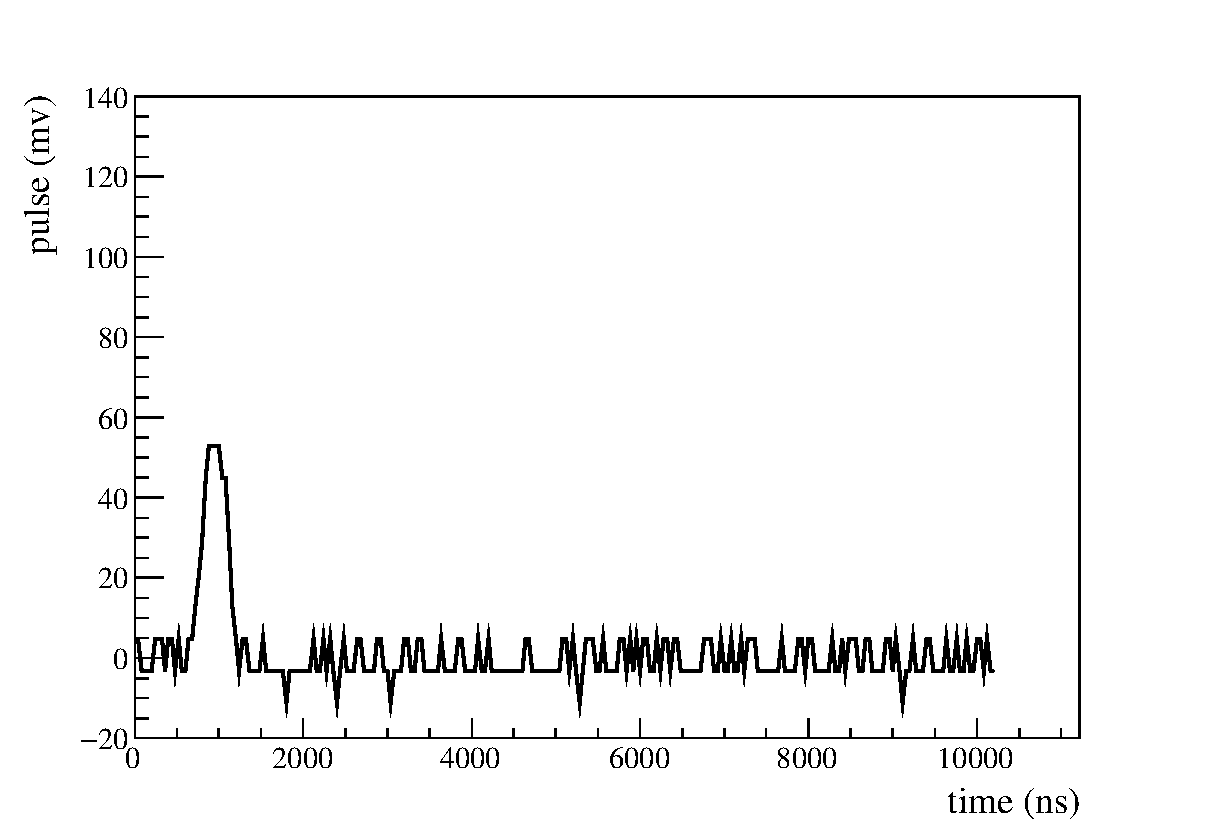
\includegraphics[clip, width=0.8\columnwidth]{0210_waveform_2.eps}
  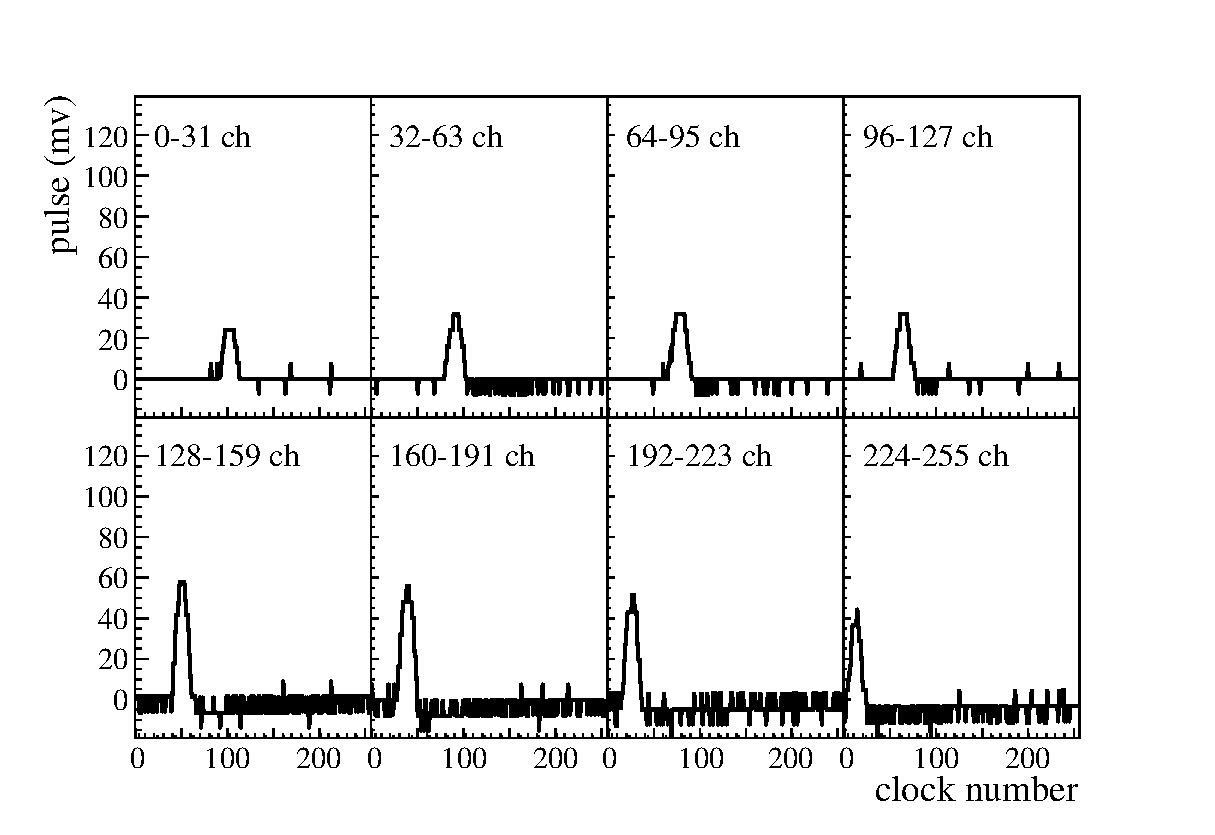
\includegraphics[clip, width=0.8\columnwidth]{0176_waveform_all_1.eps}
  \caption[FADCで取得された$\mu$-PICの波形の一例.]
          {FADCで取得された$\mu$-PICの波形の一例.
          この波形は図\ref{fig::track_demo}のanode 側の信号である.}
  \label{fig::FADC_waveform}
\end{figure}

\section{検出ガスの選出}
\label{sec::detection_gas_candidate}
標的に${}^{12}\mathrm{C}$を用いるため,分子中に炭素を含むガスを検出ガスに用いる必要がある.
${}^{12}\mathrm{C}$以外の原子核が含まれると背景事象となるが,
陽子または${}^{4}\mathrm{He}$と\SI{14}{\mega\electronvolt}の中性子の散乱では複数の荷電粒子に崩壊しないため,
トラックの本数から背景事象を取り除くことができる.
そこで,水素と炭素以外の原子が含まれない炭化水素を検出ガスに用いる.
代表的な炭化水素に,メタン (\Methane) やエタン ($\mathrm{C_{2}H_{6}}$),
イソブタン (\isoButane) がある.
また,水素ガスやヘリウムガスと炭化水素の混合ガスも用いることができる.
検出ガスとして求められる性能には以下のようなものがある.
\begin{itemize}
\item
  放電しにくい.(安定なTPC の運用)
\item
  $\alpha$粒子のエネルギー損失 ($dE/dx$) が適切である.(トラックを正しく抽出)
\item
  適切なドリフト速度を達成できる.(有感領域を効率的に使用)
\item
  電子の拡散効果が小さい.(複数のトラックを正しく抽出)
\item
  測定を行うのに十分な量の${}^{12}\mathrm{C}$を含む.(散乱標的の量)
\end{itemize}
これらの項目を基準に検出ガスの種類と圧力を決定する.

\subsection{$\alpha$粒子のエネルギー損失}
MAIKo TPC では荷電粒子のトラックの長さと方向からエネルギーと運動量を決定するため,
取得した画像からトラックを正しく抽出することが必要となる.
荷電粒子のエネルギー損失 ($dE/dx$) が大きくなりすぎると検出ガス中での飛行距離が短くなり,
トラックとして識別することが難しくなる.
また,$dE/dx$ が小さくなりすぎると荷電粒子が有感領域で停止せず,
トラックの長さを決定することができなくなる.
そこで,検出する対象である$\alpha$粒子の $dE/dx$ が適切な大きさとなるガスの種類と圧力の候補を決定する必要がある.

まず,代表的な炭化水素である\Methane を考える.
${}^{12}\mathrm{C}(0_2^+)$からの崩壊$\alpha$粒子が,ガス中で\SI{10}{\milli\metre} 以上飛行し,
MAIKo TPC の有感領域中で停止するとき,その$\alpha$粒子を検出可能な$\alpha$粒子とする.
${}^{12}\mathrm{C}(0_2^+)$の全崩壊イベント数に対する,
3つの$\alpha$粒子が全て検出可能であるイベント数の割合を検出率とする.
%図\ref{fig::alpha_E_dist}に示したエネルギー分布の$\alpha$粒子に対する,
図\ref{fig::sig_angle_dist}に示した微分断面積の角度分布を仮定したときの
検出率の圧力依存性を図\ref{fig::efficiency_P_dist}に示す.
$\alpha$粒子の飛程の計算にはSRIM~\cite{SRIM}を用いた.
SRIM は,荷電粒子がが物質中を通過する際の,イオンの飛程,エネルギーロス等を算出するシミュレーションソフトウェアである.
また,ビーム軸が有感領域の中央を通り,散乱点がビーム軸上に一様に分布していると仮定した.
図\ref{fig::efficiency_P_dist}から分かるように,\SI{50}{\hecto\pascal} で検出率が最大となっている.
%\SI{50}{\hecto\pascal}のときの\Methane の各種の値は表\ref{tab::CH4_50_params}のとおりである.
\SI{50}{\hecto\pascal}のときの\Methane の$dE/dx$と同程度となる,他の検出ガスを考え,
表\ref{tab::mixture}に示した6つを検出ガスの候補とした.
%混合ガスでは圧力を\SI{100}{\hecto\pascal} に固定し混合比をパラメータとして$dE/dx$を合わせる.
括弧内はガスの混合の割合を示す.
これらの6種類の候補から検出ガスを選ぶ.
\begin{figure}
  \centering
  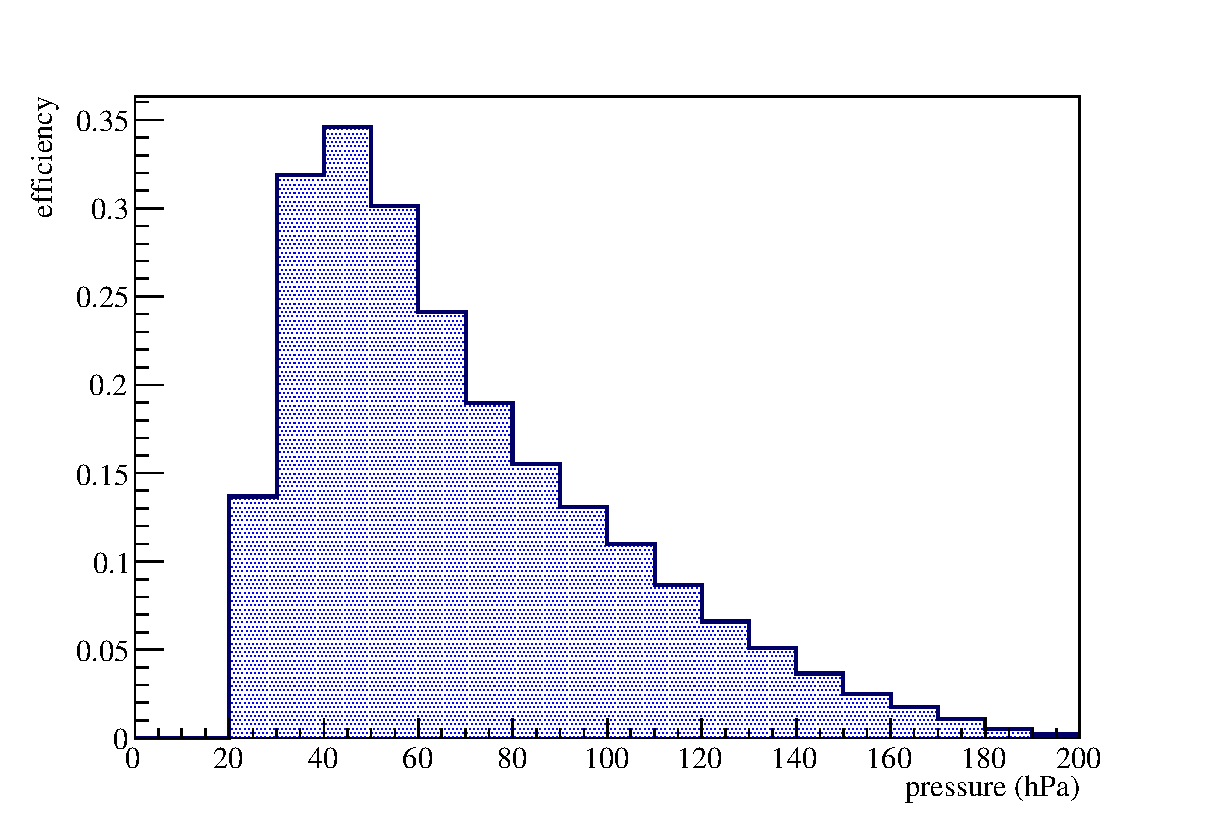
\includegraphics[clip, width=0.8\columnwidth]{efficiency_P_dist.eps}
  \caption[\Methane の圧力による検出効率の分布.]
          {\Methane の圧力による検出効率の分布.
            $\alpha$粒子は図\ref{fig::sig_angle_dist}に示した微分断面積の角度分布を仮定した.
           }
  \label{fig::efficiency_P_dist}
\end{figure}
%\begin{table}
%  \centering
%  \caption{\SI{50}{\hecto\pascal}のときの\Methane のパラメータ.}
%  \label{tab::CH4_50_params}
%  \begin{tabular}{cc}
%    \toprule
%    項目 & 値\\
%    \midrule
%    密度 & \SI{3.29e-5}{\gram\per\cubic\centi\metre} \\
%    $dE/dx$ ($E_{\alpha} = \SI{0.5}{\mega\electronvolt}$, \SI{10}{\milli\metre}) & \SI{0.107}{\mega\electronvolt}\\
%    飛程 ($E_{\alpha} = \SI{0.5}{\mega\electronvolt}$) & \SI{65.6}{\milli\metre} \\
%    検出率 & \SI{48.2}{\percent} \\
%    \bottomrule
%  \end{tabular}
%\end{table}
\begin{table}
  \centering
  \caption[ガスの混合パターン,圧力,$dE/dx$.]
          {ガスの混合パターン,圧力,$dE/dx$.
            括弧内はガスの混合の割合を示す.
            エネルギー損失は$E_{\alpha}$が\SI{0.5}{\mega\electronvolt}の$\alpha$粒子が\SI{10}{\milli\metre}で
            落とすエネルギーを表す.
            電場はMagboltz~\cite{magboltz}による計算でドリフト速度が\SI{0.014}{\milli\metre\per\nano\second}となる値である.
          }
  \label{tab::mixture}
  \begin{tabular}{ccccc}
    \toprule
    gas &
    \begin{tabular}{c}
      pressure \\
      (\si{\hecto\pascal})
    \end{tabular} &
    \begin{tabular}{c}
      density \\
      (\si{\gram\per\cubic\centi\metre})
    \end{tabular} &
    \begin{tabular}{c}
      $dE/dx$ \\
      (\si{\mega\electronvolt})% \\      
%      $E_{\alpha} = \SI{0.5}{\mega\electronvolt}$% \\
%      \SI{10}{\milli\metre}
    \end{tabular} &
    \begin{tabular}{c}
      %      ドリフト電場 (\si{\volt\per\milli\metre}) \\
      電場 \\
      (\si{\volt\per\milli\metre})% \\
%      @ \SI{0.014}{\milli\metre\per\nano\second}
    \end{tabular}\\
    \midrule
    \Methane         & 50  & 3.29$\times 10^{-5}$ & 0.107 & 0.418 \\
    \MethaneHydro    & 100 & 2.55$\times 10^{-5}$ & 0.107 & 4.31 \\
    \MethaneHerium   & 100 & 3.62$\times 10^{-5}$ & 0.109 & 1.89 \\
    \isoButane       & 15  & 3.58$\times 10^{-5}$ & 0.102 & 0.644 \\
    \isoButaneHydro  & 100 & 3.13$\times 10^{-5}$ & 0.122 & 6.80 \\
    \isoButaneHerium & 100 & 3.86$\times 10^{-5}$ & 0.102 & 3.26 \\
    \bottomrule
  \end{tabular}
\end{table}

\subsection{ドリフト速度}
MAIKo TPC では\SI{100}{\mega\hertz}で1,024 samples データを取得するため,
ドリフト方向には\SI{10.24}{\micro\second}のタイムウィンドウが開いている.
ドリフトケージの大きさ (\SI{140}{\milli\metre}) を可能な限りタイムウィンドウに収めるためには,
ドリフト速度を$\SI{140}{\milli\metre}/\SI{10.24}{\micro\second} \sim \SI{0.014}{\milli\metre\per\nano\second}$
に調整する必要がある.
Magboltz~\cite{magboltz} によって求めたドリフト電場とドリフト速度の関係を図\ref{fig::drift_v_magboltz}に示す.
ドリフト速度が\SI{0.014}{\milli\metre\per\nano\second}となるドリフト電場の値を表\ref{tab::mixture}に示す.
図\ref{fig::drift_v_magboltz}の横方向の点線は\SI{0.014}{\milli\metre\per\nano\second}を表す.
以降,これらのドリフト電場で評価を行う.
\begin{figure}
  \centering
  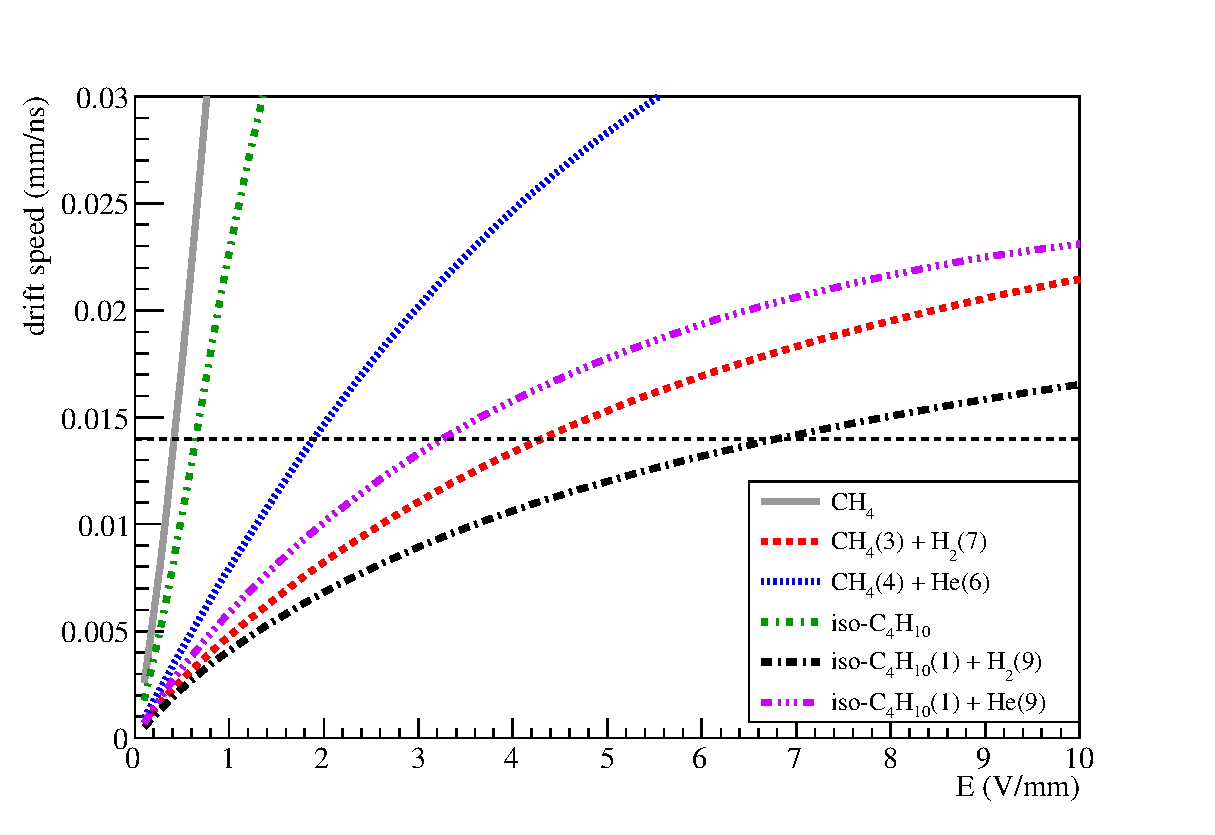
\includegraphics[clip, width=0.9\columnwidth]{drift_v_magboltz.eps}
  \caption[ドリフト電場とドリフト速度の関係.]
          {ドリフト電場とドリフト速度の関係.
            \Methane は\SI{50}{\hecto\pascal},\isoButane は\SI{15}{\hecto\pascal},その他は\SI{100}{\hecto\pascal}である.
            横方向の破線は\SI{0.014}{\milli\metre\per\nano\second}を示す.}
          \label{fig::drift_v_magboltz}
\end{figure}

\subsection{電子の拡散の効果}
ドリフト電場によって電子が移動する間に検出ガスとの散乱と電子の熱運動により,
図\ref{fig::diffusion-image}のように電子は拡散しつつドリフトする.
%電子が広がることを拡散と呼ぶ.
この効果が大きくなると,図\ref{fig::diffusion-image}の左のように
荷電粒子によって同じ場所に生成された電子が読み出し面に到達するまでに拡散する,
トラックが太く検出される.
トラックが太くなると,${}^{12}\mathrm{C}(0_2^+)$から崩壊した3つの$\alpha$粒子のトラックを分離することが難しくなる.
そのため,図\ref{fig::diffusion-image}の右のように拡散の効果が小さいことが望まれる.
\begin{figure}
  \centering
  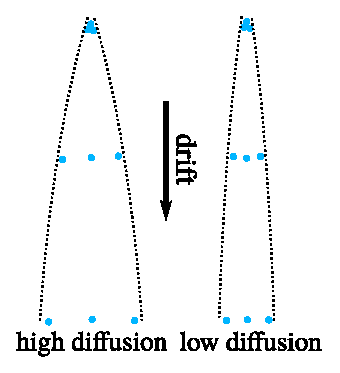
\includegraphics[clip, width=0.4\columnwidth]{diffusion_image.eps}
  \caption[電子が拡散するイメージ.]
          {電子が拡散するイメージ.
          同じ位置で生成された電子でもドリフトする間に位置が拡散する.}
  \label{fig::diffusion-image}
\end{figure}

文献~\cite{leo}によるとドリフト電場がない場合の電子の拡散は以下のように理解できる.
電子は熱運動により発生点から拡散する.
熱運動の平均速度$v$はMaxwell 分布より
\begin{equation}
  v = \sqrt{\frac{8k_{B}T}{\pi \si{\electronmass}}}
  \label{eq::maxwell_velocity}
\end{equation}
と表せる.
ここで$k_{B}$はボルツマン定数,$T$は温度,\si{\electronmass}は電子の質量である.
電子が発生した時刻から$\Delta t$後では,
\begin{equation}
  \frac{N_0}{\sqrt{4\pi D \Delta t}}\exp\left(-\frac{x^{2}}{4 D \Delta t}\right)
  \label{eq::gaus_dist}
\end{equation}
のガウス分布で電子が広がる.
ここで$N_{0}$は全粒子数,$x$は発生した点からの距離,$D$は拡散係数を表す.
拡散係数$D$は電子の平均自由行程$\lambda$を用いて
\begin{equation}
  D = \frac{1}{3}v\lambda
  \label{eq::diffusion_coef}
\end{equation}
と表せる.
これは電子の速度が遅いほど,ガスとの散乱が少ないほど遠くまで移動できるため,
拡散の効果が大きくなることを表す.
理想気体において平均自由工程$\lambda$は,ガスとの散乱の全断面積$\sigma_{0}$,圧力$p$のもとで
\begin{equation}
  \lambda = \frac{1}{\sqrt{2}}\frac{k_{B}T}{\sigma_{0}p}
  \label{eq::lambda}
\end{equation}
と表される.
式\ref{eq::maxwell_velocity}, \ref{eq::diffusion_coef}, \ref{eq::lambda}により,
\begin{equation}
  D = \frac{2}{3\sqrt{\pi}}\frac{1}{p\sigma_{0}}\sqrt{\frac{\left(k_{B}T\right)^{3}}{\si{\electronmass}}}
  \label{eq::diffusion_coef_2}
\end{equation}
となる.
式\ref{eq::diffusion_coef_2}より,
同じガスでは圧力が高いほど,温度が低いほど拡散係数が小さいことが分かる.

ドリフト電場がある場合,発生点からの距離を$L$,ドリフト速度を$v_{\text{drift}}$とすると,
\begin{equation}
  \Delta t = \frac{L}{v_{\text{drift}}}
  \label{eq::delta_t}
\end{equation}
となる.
距離$L$における分散$\sigma(L)$は
\begin{align}
  \sigma(L) & = \sqrt{2 D \Delta t}\\
  & = \sqrt{\frac{2 D}{v_{\text{drift}}}}\times\sqrt{L}\\
  & = D_{\mathrm{Magboltz}}\times\sqrt{L} \label{eq::diffusion_coef}
\end{align}
となる.
計算コードMagboltz~\cite{magboltz}によって得られた拡散係数 ($D_{\mathrm{Magboltz}}$) を表\ref{tab::diffusion}に示す.
表\ref{tab::diffusion}中の$D_{t}$はドリフト電場に対して垂直な方向への拡散,$D_{l}$は平行な方向への拡散の係数を表す.
\Methane および\isoButane の単体では拡散係数が大きく,
同じドリフト速度のとき,ドリフト電場が大きいほど拡散係数が小さいことが分かる.
\isoButaneHydro の拡散係数が最も小さく,
検出ガスの最有力候補である.
次章ではシミュレーションにより生成した${}^{12}\mathrm{C}(\mathrm{n},\mathrm{n}'){}^{12}\mathrm{C} (0_2^+)$イベントを解析し,
その解析効率により検出ガスを決定する.
\begin{table}
  \centering
  \caption[Magboltz で計算した拡散係数.]
          {Magboltz で計算した拡散係数.
            拡散の大きさはドリフト電場に依存するため,
            ここではドリフト速度が\SI{0.014}{\milli\metre\per\nano\second}になるドリフト電場での値を示す.
          $D_{t}$,$D_{l}$はそれぞれ運動方向に垂直,平行方向の拡散係数.}
  \label{tab::diffusion}
  \begin{tabular}{ccccc}
    \toprule
    gas & 圧力 (\si{\hecto\pascal}) & $D_{t}$ (\si{\sqrt{\milli\metre}}) & $D_{l}$ (\si{\sqrt{\milli\metre}}) &
    \begin{tabular}{c}
      ドリフト電場 \\
      (\si{\volt\per\milli\metre})
    \end{tabular}\\
    \midrule
    \Methane & 50 & 0.433 & 0.547 & 0.418\\
    \MethaneHydro & 100 & 0.214 & 0.171 & 4.31\\
    \MethaneHerium & 100 & 0.270  & 0.248 & 1.89\\
    \isoButane & 15 & 0.357 & 0.414 & 0.644\\
    \isoButaneHydro & 100 & 0.196 & 0.145 & 6.80\\
    \isoButaneHerium & 100 & 0.246 & 0.197 & 3.26\\
    \bottomrule
  \end{tabular}
\end{table}

%\section{$\alpha$線源を用いた測定}
%$\alpha$線源を用いてMAIKo TPC の動作確認を行う.
%線源では,電子のドリフトスピード,増幅率,トラックの太さを確認する.

%\subsection{HV系}
%%ここでは電圧の変数名を説明する.
%
%\subsection{ガス系}
%
%\subsection{回路系}
%

%ドリフト速度の決定方法は30 degree 方向に$\alpha$線源から$\alpha$を出して,
%その飛跡がデータ上でどう見えるかで決定する.
%ドリフト速度の時間依存性も見た.

%\section{中性子カウンター (液体シンチレータ)}
%\subsection{キャリブレーション}
%\subsection{波形弁別}
%\subsection{検出効率}
%
%\section{中性子カウンター (金属箔)}
%

\end{document}
